\section{Einführung in das modulare Bad}\label{sec:sanMOD}

\textbf{Im folgenden zitieren wir die Website des Auftraggebers \\die {\projectpartner}} \cite{SanMOD} \\
\textit{
Jedes SanMOD-Bad besteht aus 3 Modulen: \\
Einem WC-Modul, einem Dusch-Modul und einem Waschtischmodul. Die Anordnung der Module ist flexibel und richtet sich sowohl nach den \\räumlichen Vorgaben als auch nach der gewünschten Offenheit des Badezimmers zum restlichen Raum hin. Der Grundaufbau jedes SanMOD-Bades besteht aus vorgefertigten TECEsystem-Wandelementen die bereits alle Verrohrungen und Verkabelungen sowie einen hochwertigen TECE-Spülkasten enthalten.
\\
Auf dieser Basiskonstruktion werden sämtliche Bestandteile eines hochwertigen Hotel-Badezimmers montiert.
}
\section*{WC-Modul}
Jedes WC-Modul beinhaltet ein komplett funktionsfähiges WC. Des Weiteren gehören auch die mit einem Design versehenen Wände dazu. Für eine angenehme Atmosphäre sorgen die in der Decke inkludierten Lüfter samt Beleuchtung.

\begin{figure}[h]
    \centering
    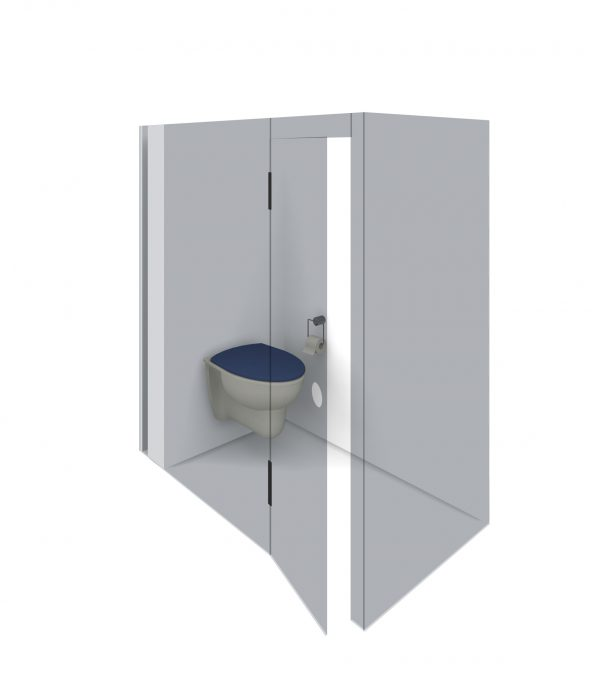
\includegraphics[width=0.6\textwidth]{images/Modul-WC-600x676.jpg}
    \caption{Ein Beispiel wie ein WC-Modul aussieht \cite{SanMOD}}
    \label{}
\end{figure}
    

\section*{Duschmodul}
Alle Duschmodule sind mit dem für den Kunden angefertigten Design versehen und sorgen gemeinsam mit den Deckenelementen wie zum Beispiel den Lüfter und Lichter für ein ideales Ambiente. Die Duschen sind allesamt betriebsfertig und beinhalten alle benötigte Elementen.

\begin{figure}[h]
    \centering
    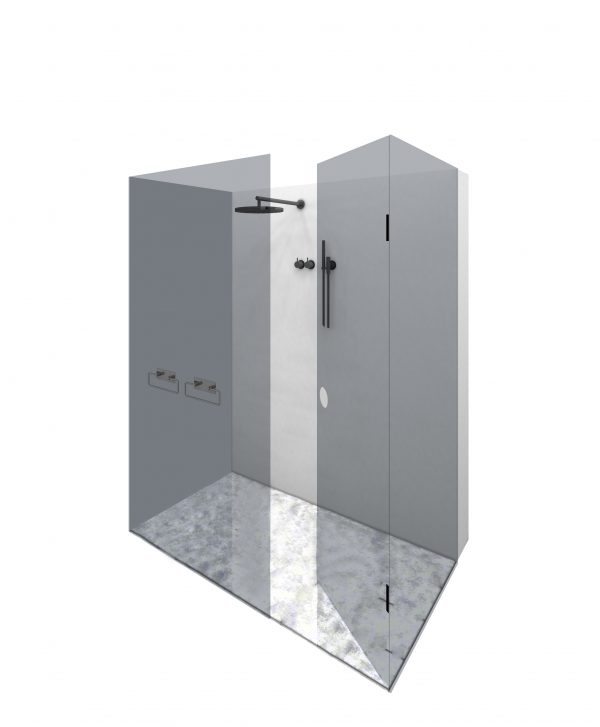
\includegraphics[width=0.8\textwidth]{images/Modul-Dusche-600x727.jpg}
    \caption{Ein Beispiel wie ein Duschmodul aussieht \cite{SanMOD}}
    \label{}
\end{figure}
    
\clearpage
\newpage
\section*{Waschtischmodul}\label{sec:waschtischmodul}
Die Waschtischmodule implizieren alle für die Verwendung benötigten Sanitäranlagen. Ein Spiegel mit Beleuchtung gehört zur Standardausstattung. Darüber hinaus ist ein FanCoil fixer Bestandteil jedes SanMOD-Bades und sorgt damit für perfekte Klimatisierung jedes Hotelzimmers.

\begin{figure}[h]
    \centering
    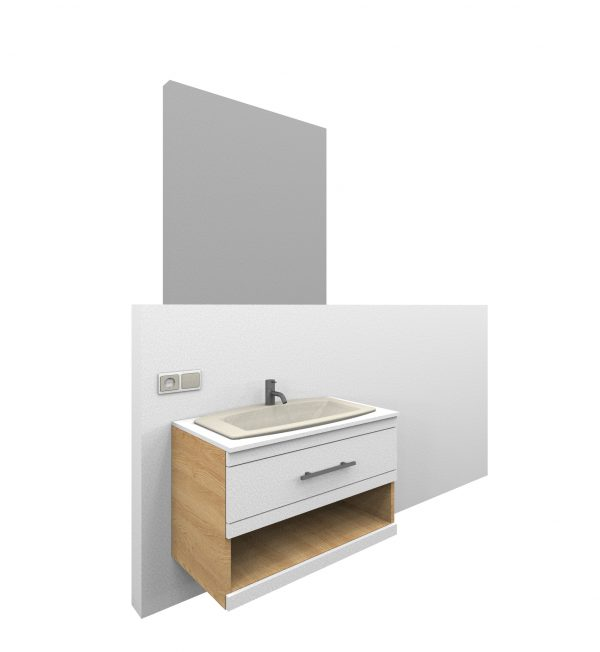
\includegraphics[width=0.8\textwidth]{images/Modul-Waschtisch-600x652.jpg}
    \caption{Ein Beispiel wie ein Waschtischmodul aussieht \cite{SanMOD}}
    \label{}
\end{figure}    
